\chapter{Teoria sulla complessità}
\section{La funzione tempo di esecuzione}
Dato un qualsiasi algoritmo, è possibile ottenere la funzione $T(n)$ ad esso associata, ossia la \textbf{funzione tempo di esecuzione} rispetto alla dimensione dell'input $n$. Questa funzione prende in considerazione solamente il numero di istruzioni e non aspetti dinamici d'esecuzione.\\
Studiando l'andamento asintotico di $T(n)$, si può notare che è rilevante ciò che cresce più velocemente:
\textit{es} $T(n)=a+bn+cn^2 \Rightarrow T(n) = \varTheta(n^2)$.
\subsection*{Il caso peggiore, migliore e medio}
Si possono costruire \textit{tre} funzioni $T(n)$ per stimare l'efficienza dei un programma:
\begin{itemize}[noitemsep, nolistsep]
	\item $T_\text{peggiore}(n)$ nel caso peggiore
	\item $T_\text{migliore}(n)$ nel caso migliore
	\item $T_\text{medio}(n)$ nel caso medio
\end{itemize}
\vspace{10px}
Di ciascuna di esse si può determinare l'andamento asintotico attraverso le notazioni successivamente fornite.

\section{Notazione per l'andamento asintotico}
\subsection*{Notazione limite superiore $O$-grande}
\begin{gather*}
f(n)=O(g(n))\\
\text{se } \exists n_0 >0, \exists c_2 >0 \text{ tc. } f(n)\leq c_2 g(n) \forall n>n_0
\end{gather*}

\subsection*{Notazione limite inferiore $\varOmega$-omega}
\begin{gather*}
f(n)=\varOmega(g(n))\\
\text{se } \exists n_0 >0, \exists c_1 >0 \text{ tc. } f(n)\geq c_1 g(n) \forall n>n_0
\end{gather*}

\subsection*{Notazione limite superiore e inferiore $\varTheta$-theta}
\begin{gather*}
f(n)=\varTheta(g(n))\\
\text{se } \exists n_0 >0, \exists c_1>0,c_2>0 \text{ tc. } c_1g(n)\leq f(n)\leq c_2 g(n) \forall n>n_0
\end{gather*}

\section{Definizione di complessità}

\paragraph{Complessità di un algoritmo} La complessità di un algoritmo equivale alla misura del numero di istruzioni da eseguire per risolvere il problema.

\paragraph{Complessità di un problema} La complessità di un problema equivale alla complessità del migliore algoritmo che lo risolve.

\section{Le equazioni di ricorrenza}
Quando si deve analizzare un algoritmo ricorsivo del tipo \textit{divide et impera}, non è possibile scrivere l'espressione analitica di $T(n)$. Bisogna utilizzare un'equazione di ricorrenza:
\begin{equation*}
T(n) = 
\begin{cases}
\varTheta(1), n\le c\\
aT\Bigl(\frac{n}{b}\Bigr)+D(n)+C(n), n>c
\end{cases}
\end{equation*}
Dove:
\begin{itemize}[noitemsep, nolistsep]
	\item $c$ costante
	\item $a$ numero di problemi generati da \textit{divide}
	\item $b$ dimensione dei sottoproblemi rispetto a quello originale
	\item $D(n)$ tempo impiegato per dividere il sottoproblema (operazione di \textit{divide})
	\item $C(n)$ tempo impiegato per ricombinare le soluzioni dei sottoproblemi (operazione di \textit{combina})
\end{itemize}

\section{Risoluzione delle equazioni di ricorrenza}

\subsection{Metodo iterativo}
Questo metodo consiste nel calcolare $T(n)$ in funzione delle sue iterazioni successive.
\paragraph{Esempio}

\begin{flalign*}
&\begin{cases}
T(1) = 1\\
T(n) = 1 + T(\frac{n}{2})
\end{cases}\\
&\hspace{30px}T\Bigl(\frac{n}{2}\Bigr) = T\Bigl(\frac{n}{4}\Bigr)+1
\quad T\Bigl(\frac{n}{4}\Bigr) = T\Bigl(\frac{n}{8}\Bigr)+1 \hspace{\linewidth}\\
&\hspace{30px}T(n) = T\Bigl(\frac{n}{4}\Bigr)+1+1\\
&\hspace{30px}T(n) = T\Bigl(\frac{n}{8}\Bigr)+1+1+1
\end{flalign*}
Dunque, alla \textit{i}-esima iterazione: $T(n)=T\bigl(\frac{n}{2^i}\bigr)+i$\\
Per ottenere il limite asintotico superiore, ci si ferma quando: $\frac{n}{2^i}=1 \Rightarrow n=2^i \Rightarrow i=\log_2n$\\
\begin{equation*}
T(n) = T(1)+\log_2n= 1+\log_2n \Rightarrow T(n)=O(\log_2n)
\end{equation*}

\subsection{Metodo dell'esperto}
Si definisce il seguente teorema:
\begin{gather*}
a,b\in\mathbb{N}, a\ge1, b\ge2, c\in\mathbb{R}, \beta\in\mathbb{R}, c\ge0, \beta\ge0\\
T(n)=
\begin{cases}
aT\bigl(\frac{n}{b}\bigr)+cn^\beta, n>1\\
d, n\le1
\end{cases}
\end{gather*}
Posto $\alpha = \log_ba = \frac{\log a}{\log b}$, si ha che:
\begin{equation*}
T(n) = 
\begin{cases}
\varTheta(n^\alpha), \alpha>\beta\\
\varTheta(n^\alpha\log_2n), \alpha=\beta\\
\varTheta(n^\beta), \alpha<\beta
\end{cases}
\end{equation*}

\subsection{Metodo dell'albero di ricorsione}

\paragraph{Esempio}
\begin{flalign*}
T(n) = 
&\begin{cases}
\varTheta(1), n\le c\\
3T(\frac{n}{4})+\varTheta(n^2), n>c
\end{cases}
\end{flalign*}

\begin{center}
	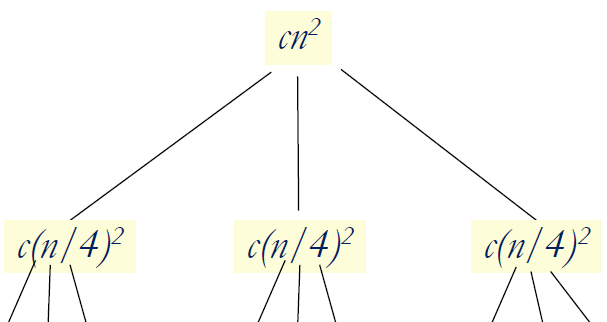
\includegraphics[width=0.5\textwidth]{img/albero_di_ricorsione.png}
\end{center}

\begin{enumerate}[noitemsep]
	\item si calcola il numero dei nodi per livello: $3^i$ in questo caso.
	\item si calcola il peso di ciascun livello moltiplicando il numero di nodi per livello per il peso di ciascun nodo di quel livello
	\item si calcola il numero di livelli: $log_4n+1$ in questo caso. Si noti che il $4$ è il valore di $b$ dell'equazione di ricorrenza. Il numero dei livelli deve essere dimostrato per induzione.
	\item si calcola il numero di foglie: in questo caso $3^\text{altezza}$, dove l'altezza dell'albero è il numero di livelli meno 1.
	\item T(n) è pari dunque alla somma dei pesi di $i-1$ livelli più la somma dei pesi delle foglie.
\end{enumerate}

\subsection{Metodo della sostituzione}
Per applicare il metodo di sostituzione:
\begin{enumerate}
	\item si indovini la soluzione $\varTheta(f(n))$ (si consiglia il metodo dell'esperto).
	\item dimostrare per induzione la validità del limite superiore, inferiore o entrambi in base alla richiesta.
\end{enumerate}

\paragraph{Esempio}
\begin{flalign*}
&\begin{cases}
T(1) = 1\\
T(n) = n + 2T(\frac{n}{2})
\end{cases}
\end{flalign*}
Si ha: $T(n) = \varTheta(n\log_2n) \Rightarrow c_1n\log_2n\le T(n) \le c_2n\log_2n $ per il teorema dell'esperto.\\
Si studia il limite superiore trovando per quali $c>0$ vale $T(n) \le c_2n\log_2n$:
\begin{enumerate}[noitemsep, nolistsep]
	\item Si prova il caso base tramite il principio dell'induzione.
	\item Si utilizza l'ipotesi induttiva: $k<n, T(k)\le ck\log_2k$.
\end{enumerate}
Quindi: $T(n)=2T(\frac{n}{2})+n \le 2c\frac{n}{2}\log_2\frac{n}{2}+n$, e così via.\\
Per il limite inferiore il procedimento è del tutto analogo:
\begin{enumerate}[noitemsep, nolistsep]
	\item Si prova il caso base tramite il principio dell'induzione.
	\item Si utilizza l'ipotesi induttiva: $k<n, T(k)\ge dk\log_2k$.
\end{enumerate}